%%%%%%%%%%%%%%%%%%%%%%%%%%%%%%%%%%%%%%%%%%%%%%%%%%%%%%%%%%%%%%%%%%%%%%%%%%%
%% This file is part of the book
%%
%% Algorithmic Graph Theory
%% http://code.google.com/p/graph-theory-algorithms-book/
%%
%% Copyright (C) 2009, 2010, 2011 Minh Van Nguyen <nguyenminh2@gmail.com>
%%
%% See the file COPYING for copying conditions.
%%%%%%%%%%%%%%%%%%%%%%%%%%%%%%%%%%%%%%%%%%%%%%%%%%%%%%%%%%%%%%%%%%%%%%%%%%%

\documentclass{article}

\usepackage{subfigure}
\usepackage{tikz}
\usetikzlibrary{external}
\usetikzlibrary{trees}
\tikzexternalize{binary-search-tree-delete}

\begin{document}

\begin{figure}
\subfigure[Target vertex $9$ is a leaf.]{
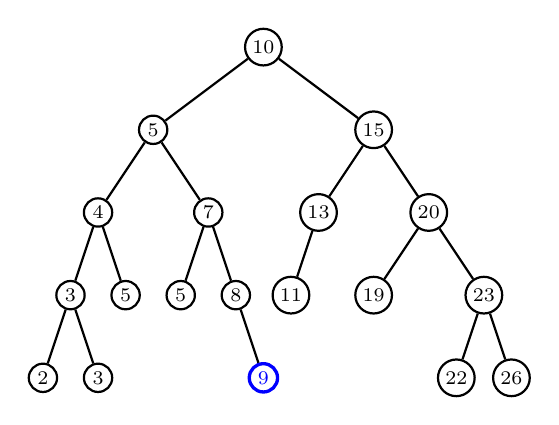
\begin{tikzpicture}
[-,thick,%
  every node/.style={shape=circle,inner sep=1.5pt,draw,thick},%
  scale=0.7]
\scriptsize
\node {$10$}
  [sibling distance=4cm]
  child {node {$5$}
    [sibling distance=2cm]
    child {node {$4$}
      [sibling distance=1cm]
      child {node {$3$}
        child {node {$2$}}
        child {node {$3$}}
      }
      child {node {$5$}}
    }
    child {node {$7$}
      [sibling distance=1cm]
      child {node {$5$}}
      child {node {$8$}
        child[missing]
        child {node[blue,very thick] {$9$}}
      }
    }
  }
  child {node {$15$}
    [sibling distance=2cm]
    child {node {$13$}
      [sibling distance=1cm]
      child {node {$11$}}
      child[missing]
    }
    child {node {$20$}
      child {node {$19$}}
      child {node {$23$}
        [sibling distance=1cm]
        child {node {$22$}}
        child {node {$26$}}
      }
    }
  };
\end{tikzpicture}
}
%%
%%
\qquad
\subfigure[Leaf deleted.]{
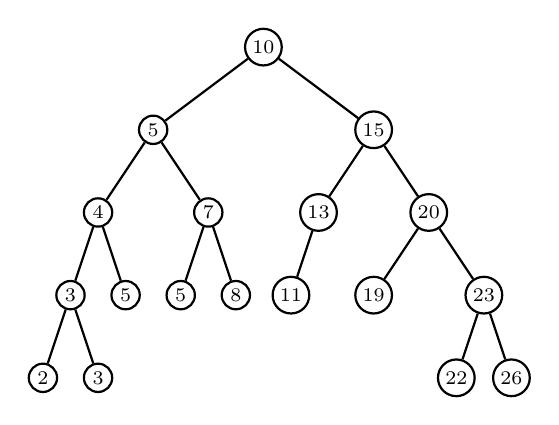
\begin{tikzpicture}
[-,thick,%
  every node/.style={shape=circle,inner sep=1.5pt,draw,thick},%
  scale=0.7]
\scriptsize
\node {$10$}
  [sibling distance=4cm]
  child {node {$5$}
    [sibling distance=2cm]
    child {node {$4$}
      [sibling distance=1cm]
      child {node {$3$}
        child {node {$2$}}
        child {node {$3$}}
      }
      child {node {$5$}}
    }
    child {node {$7$}
      [sibling distance=1cm]
      child {node {$5$}}
      child {node {$8$}}
    }
  }
  child {node {$15$}
    [sibling distance=2cm]
    child {node {$13$}
      [sibling distance=1cm]
      child {node {$11$}}
      child[missing]
    }
    child {node {$20$}
      child {node {$19$}}
      child {node {$23$}
        [sibling distance=1cm]
        child {node {$22$}}
        child {node {$26$}}
      }
    }
  };
\end{tikzpicture}
}
%%
%%
\subfigure[Target vertex $13$ has one child.]{
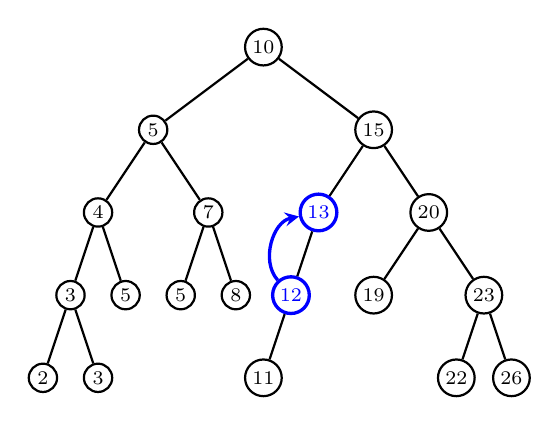
\begin{tikzpicture}
[-,thick,%
  every node/.style={shape=circle,inner sep=1.5pt,draw,thick},%
  scale=0.7]
\scriptsize
\node {$10$}
  [sibling distance=4cm]
  child {node {$5$}
    [sibling distance=2cm]
    child {node {$4$}
      [sibling distance=1cm]
      child {node {$3$}
        child {node {$2$}}
        child {node {$3$}}
      }
      child {node {$5$}}
    }
    child {node {$7$}
      [sibling distance=1cm]
      child {node {$5$}}
      child {node {$8$}}
    }
  }
  child {node {$15$}
    [sibling distance=2cm]
    child {node[blue,very thick] (13) {$13$}
      [sibling distance=1cm]
      child {node[blue,very thick] (12) {$12$}
        child {node {$11$}}
        child[missing]
      }
      child[missing]
    }
    child {node {$20$}
      child {node {$19$}}
      child {node {$23$}
        [sibling distance=1cm]
        child {node {$22$}}
        child {node {$26$}}
      }
    }
  };
\path
(12) edge[->,>=stealth,blue,very thick,bend left=60] (13);
\end{tikzpicture}
}
%%
%%
\qquad
\subfigure[Vertex deleted.]{
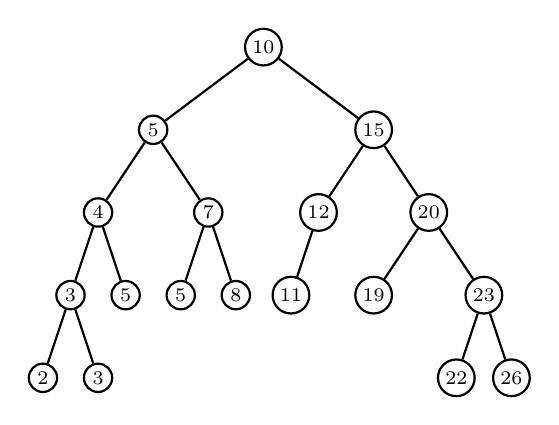
\begin{tikzpicture}
[-,thick,%
  every node/.style={shape=circle,inner sep=1.5pt,draw,thick},%
  scale=0.7]
\scriptsize
\node {$10$}
  [sibling distance=4cm]
  child {node {$5$}
    [sibling distance=2cm]
    child {node {$4$}
      [sibling distance=1cm]
      child {node {$3$}
        child {node {$2$}}
        child {node {$3$}}
      }
      child {node {$5$}}
    }
    child {node {$7$}
      [sibling distance=1cm]
      child {node {$5$}}
      child {node {$8$}}
    }
  }
  child {node {$15$}
    [sibling distance=2cm]
    child {node {$12$}
      [sibling distance=1cm]
      child {node {$11$}}
      child[missing]
    }
    child {node {$20$}
      child {node {$19$}}
      child {node {$23$}
        [sibling distance=1cm]
        child {node {$22$}}
        child {node {$26$}}
      }
    }
  };
\end{tikzpicture}
}
%%
%%
\subfigure[Target vertex $15$ has two children.]{
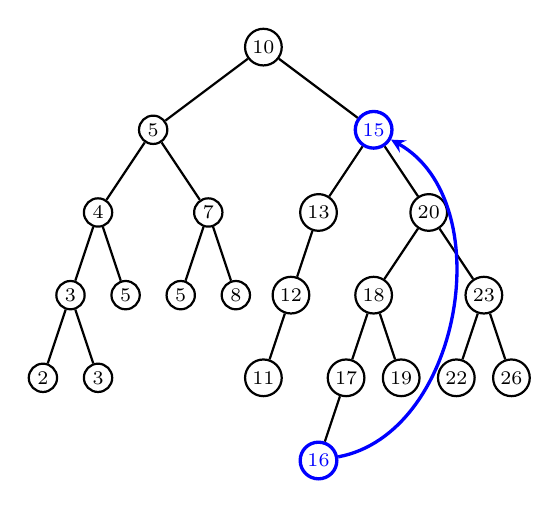
\begin{tikzpicture}
[-,thick,%
  every node/.style={shape=circle,inner sep=1.5pt,draw,thick},%
  scale=0.7]
\scriptsize
\node {$10$}
  [sibling distance=4cm]
  child {node {$5$}
    [sibling distance=2cm]
    child {node {$4$}
      [sibling distance=1cm]
      child {node {$3$}
        child {node {$2$}}
        child {node {$3$}}
      }
      child {node {$5$}}
    }
    child {node {$7$}
      [sibling distance=1cm]
      child {node {$5$}}
      child {node {$8$}}
    }
  }
  child {node[blue,very thick] (15) {$15$}
    [sibling distance=2cm]
    child {node {$13$}
      [sibling distance=1cm]
      child {node {$12$}
        child {node {$11$}}
        child[missing]
      }
      child[missing]
    }
    child {node {$20$}
      child {node {$18$}
        [sibling distance=1cm]
        child {node {$17$}
          child {node[blue,very thick] (16) {$16$}}
          child[missing]
        }
        child {node {$19$}}
      }
      child {node {$23$}
        [sibling distance=1cm]
        child {node {$22$}}
        child {node {$26$}}
      }
    }
  };
\path
(16) edge[->,>=stealth,blue,very thick,bend right=70] (15);
\end{tikzpicture}
}
%%
%%
\qquad
\subfigure[Vertex deleted.]{
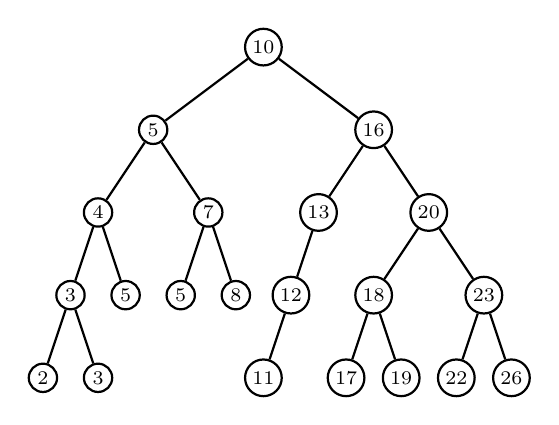
\begin{tikzpicture}
[-,thick,%
  every node/.style={shape=circle,inner sep=1.5pt,draw,thick},%
  scale=0.7]
\scriptsize
\node {$10$}
  [sibling distance=4cm]
  child {node {$5$}
    [sibling distance=2cm]
    child {node {$4$}
      [sibling distance=1cm]
      child {node {$3$}
        child {node {$2$}}
        child {node {$3$}}
      }
      child {node {$5$}}
    }
    child {node {$7$}
      [sibling distance=1cm]
      child {node {$5$}}
      child {node {$8$}}
    }
  }
  child {node {$16$}
    [sibling distance=2cm]
    child {node {$13$}
      [sibling distance=1cm]
      child {node {$12$}
        child {node {$11$}}
        child[missing]
      }
      child[missing]
    }
    child {node {$20$}
      child {node {$18$}
        [sibling distance=1cm]
        child {node {$17$}}
        child {node {$19$}}
      }
      child {node {$23$}
        [sibling distance=1cm]
        child {node {$22$}}
        child {node {$26$}}
      }
    }
  };
\end{tikzpicture}
}
\end{figure}

\end{document}
